\chapter{ASSIGNMENTS}
\vspace{0.5}
\section*{\centering\LARGE{Lab Assignment 01}}

\subsection*{\underline{Aim}}
Refer Chapter 7 of first reference to develop the problem under consideration and justify feasibility using concepts of knowledge canvas and IDEA Matrix. 
\subsection*{\underline{Project}}
Database security using Image Captcha as Graphical Password(CaGP) and Steganography.\\
\begin{table}[ht]
\caption{Project Canvas}
\begin{tabular}{ |p{5cm}|p{5cm}|p{5cm}|  }
 \hline
 \textbf{Purpose} & \textbf{Goals} & \textbf{Users}\\
 \hline
To increase safety and security & Increase the security for (captcha) Verification & Banking Sector\\

To hide data securely in video format & Store data  in video format & Verification Analysts\\
 \hline
 \end{tabular}
 \vspace{0.5cm} 
 
\begin{tabular}{ |p{5cm}|p{5cm}|p{5cm}|  }
 \hline
 \textbf{Actions} & \textbf{Deliverables} & \textbf{Risks} \\
 \hline
 Verification Login  & SRS  \& Project Design & DB may get compromised\\


  Analyze input data & Project Report \& Project & DB may leads to system error\\
   \hline
 
 \end{tabular}
 
\vspace{0.5cm} 

 \begin{tabular}{ |p{5cm}|p{5cm}|p{5cm}|  }
 \hline
 \textbf{Milestones} & \textbf{Constraints} & \textbf{Scope} \\
 \hline
 Synopsis, Abstract, Report & Input to be stored in DB & Concurrent Processing\\

  Coding and Final Software & Software must meet minimum system requirement & Password Protection \\ 
   \hline
 
 \end{tabular}

\end{table} \\\\
\pagebreak
\newpage
\noindent\\\\
\\\\
\\\\
\\\\
\\\\
\\\\
\\\\
\\\\
\\\\
\\\\
\\\\
 \newpage
\section*{\centering\LARGE{Lab Assignment 02}}
\subsection*{\underline{Aim}}
Project problem statement feasibility assessment using NP-Hard, NP-Complete or satisfy ability issues using modern algebra and/or relevant mathematical models.

\subsection*{\underline{Feasibility Theory}}
The feasibility of the project can be defined as the measure of our project whether it is viable or not.It includes various different types of feasibility as follows:
\begin{itemize}
\item \textbf{Performance:}\\
In this we check whether the proposed system is capable of performing all the functional requirements as mentioned in system features in SRS.If our system is displaying the functional requirements appropriately then it's performance is feasible.Here we also check the accuracy and efficiency of the system based on their algorithms.
\item \textbf{Technical:}\\
In this we check whether the technical specification provided that is hardware and software requirements are minimum requirements for our application software to run successfully without any error regarding the system configuration.Also the  storage requirements is quite enough and concurrency takes place effectively.
\item \textbf{Economical:}\\
In this we check the cost per line of code also the cost for storage of data and cost related to the run time of the system.Apart from this since no extra hardware is needed apart from minimum system configuration for the computers on network.


\end{itemize}
\noindent
\subsection*{\underline{Feasibility on basis of Class of Problem}}
\hspace{5em}Complexity classes are one way to talk about how difficult or easy a problem is.
Complexity theory gets very technical but the basics are actually extraordinarily
intuitive, and it's possible to understand the P versus NP issue with very little
math background.\\

\hspace{1em}If there is a fast solution to the search version of a problem then the problem is
said to be Polynomial time,
or P for short. If there is a fast solution to the verification version of a problem then the problem is said to be
Non deterministic Polynomial time,
or NP for short. The question of
"P=NP" is then the question of whether these sets are identical.\\

\hspace{1em}Some problems can be translated into one another in such a way that a fast
solution to one problem would automatically give us a fast solution to the
other. There are some problems that every single problem in NP can be
translated into, and a fast solution to such a problem would automatically give
us a fast solution to every problem in NP. This group of problems are known as
NP Hard.Some problems in NP Hard
are actually not themselves in NP,the
group of problems that are in both NP and NP Hard
is called NP Complete

\subsection*{\underline{Classes of problems}}
\begin{itemize}
\item \textbf{NP}\\
A lot of programs that don't (necessarily) run in polynomial time
on a regular computer, but do run in polynomial time on a non deterministic
Turing machine. These programs solve problems in NP, which stands for
non deterministic polynomial time.An equivalent way to define NP is by pointing to the problems that can be
verified in polynomial time.

\item \textbf{NP Hard}\\
If a problem is NP hard,
this means I can reduce any problem in NP to that problem. This means if I can solve that problem, I can easily solve any problem in NP. If we could solve an NP hard
problem in polynomial time, this would
prove P = NP.

\item \textbf{NP Complete}\\
A problem is NP complete
if the problem is both
NP hard, and in NP
\end{itemize}
\noindent
\hspace{5em}Our project  is  divided  into  two  parts.   First  part  is  login  phase  using  vi- sual cryptography scheme and second part is watermarking for upload and download data with video watermark.  As we are providing security to both login phase and data, it should not be in NP hard or np.  Our vcs algorithm will not go in infinite loop or it will not cause system to get stand by.
Same thing will happen for watermarking algorithms also.  Output of this
system will definitely come but time will not same for each output hence it is in np complete.

\subsection*{\underline{Relation Between Classes of Problems}}
 \begin{figure}[H]
    \centering
  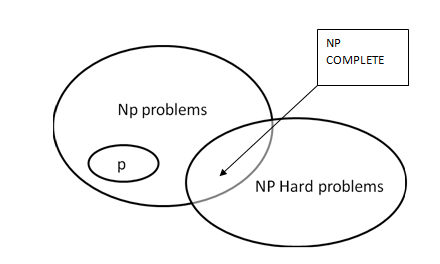
\includegraphics[scale=0.9]{np.PNG}\\
 \caption{Relation between Classes of Problems}
  
\end{figure}

\subsection*{\underline{Mathematical Model}}
 Let the M is the universal states which contains, \\
    \textbf{M = \{Q, S, F, Q0 , Qf \}} \newline
    where, \\
    		Q = No. of states \{Q0,Q1,Q2,Q3,Q4,Q5,Q6,Q7,Qf\}\\
    		Q0= Initial State.\\
    		Qf= Final State.\\
    		S= Success state.\\
    		F= Failure state.\\
    		\newline
		
    where,\\ 
    \newline
    Q0= Start.\\
     \newline
    Q1 = SignUp \\
    \newline
    Q2 = Generation of CaGP on Serverside\\
    \newline
    Q3 = Login\\
    \newline 
    Q4 = Verification of CaGP\\
    \newline
    Q5 = Select the data to be hidden\\
    \newline 
    Q6 = Select the file in which the data is to be hidden\\
    \newline
    Q7 = Steganography\\
    \newline 
    Qf = Encrypted data\\
    \newline 
    
    F = \{F,S\} \newline
    \newline Where ,
    \newline F  = Failure if the Username,Password or CaGP entered is incorrect\\
        \newline S = Successfully log in, Data is successfully Encrypted\\






\newpage
\section*{\centering\LARGE{Lab Assignment 03}}
\subsection*{\underline{Aim}}
Use of divide and conquer strategies to exploit distributed/parallel/concurrent processing of the above to identify objects, morphisms, overloading in functions (if any), and functional relations and any other dependencies (as per requirements).
\subsection*{\underline{Concept}}
A divide and conquer algorithm works by recursively breaking down a problem into two or more sub-problems of the same (or related) type (divide), until these become simple enough to be solved directly (conquer). So have divided our problem based on algorithm used and those are:
\begin{itemize}
\item Getting data from user.
\item Scene Change Detection(Compare 2 frames based on their color histogram)
\item Split Algorithm(Decide number of rows and columns to split the watermark image)
\item Least Significant Bit Algorithm(few least significant bits are substituted within data to be hidden)
\end{itemize}

\vspace*{0.4cm}
\noindent
\hspace{5em}Divide and conquer (D\&C) is an algorithm design paradigm based on multi-branched recursion. So we have to recursively divide our problem into  sub-problems  of the same (or related) type (divide), until these sub-problem become simple enough to be solved directly (conquer). The solutions to the sub-problems are then combined to give a solution to the original problem.\\

%\vspace*{0.4cm}
\noindent
\hspace{5em}In our project we are using a similar but with a slight difference in Divide and Conquer strategies in Scene change detection algo and split algo.In scene change algo we are the dividing the the file e.g video into frames and making the histograms of each frame.If the change in actual frame and the frame of the encrypted file is above the threshold then the scene is vchanged and the file is again processed until it match threshold level.
        same in case of split algo the data or the watermarke image to be hidden is divided into chunks.Number of rows and columns are decided to slit the watermark.
\newpage
\noindent
\textbf{System Specifications and Dependencies}\\
The system comprises of following major components : 
\begin{itemize}


\item SignUp/Register and Login :- take input from files.
\item Compare 2 frames based on their color histogram
\item Decide number of rows and columns to split the watermark image
\item few least significant bits are substituted within data to be hidden.
\end{itemize}

 

\newpage
\section*{\centering\LARGE{Lab Assignment 04}}
\subsection*{\underline{Aim}}
Use of above to draw functional dependency graphs and relevant Software modelling methods, techniques including UML diagrams or other necessities using appropriate tools.
    \subsection*{USE CASE DIAGRAM}
    \begin{figure}[H]
    \centering
  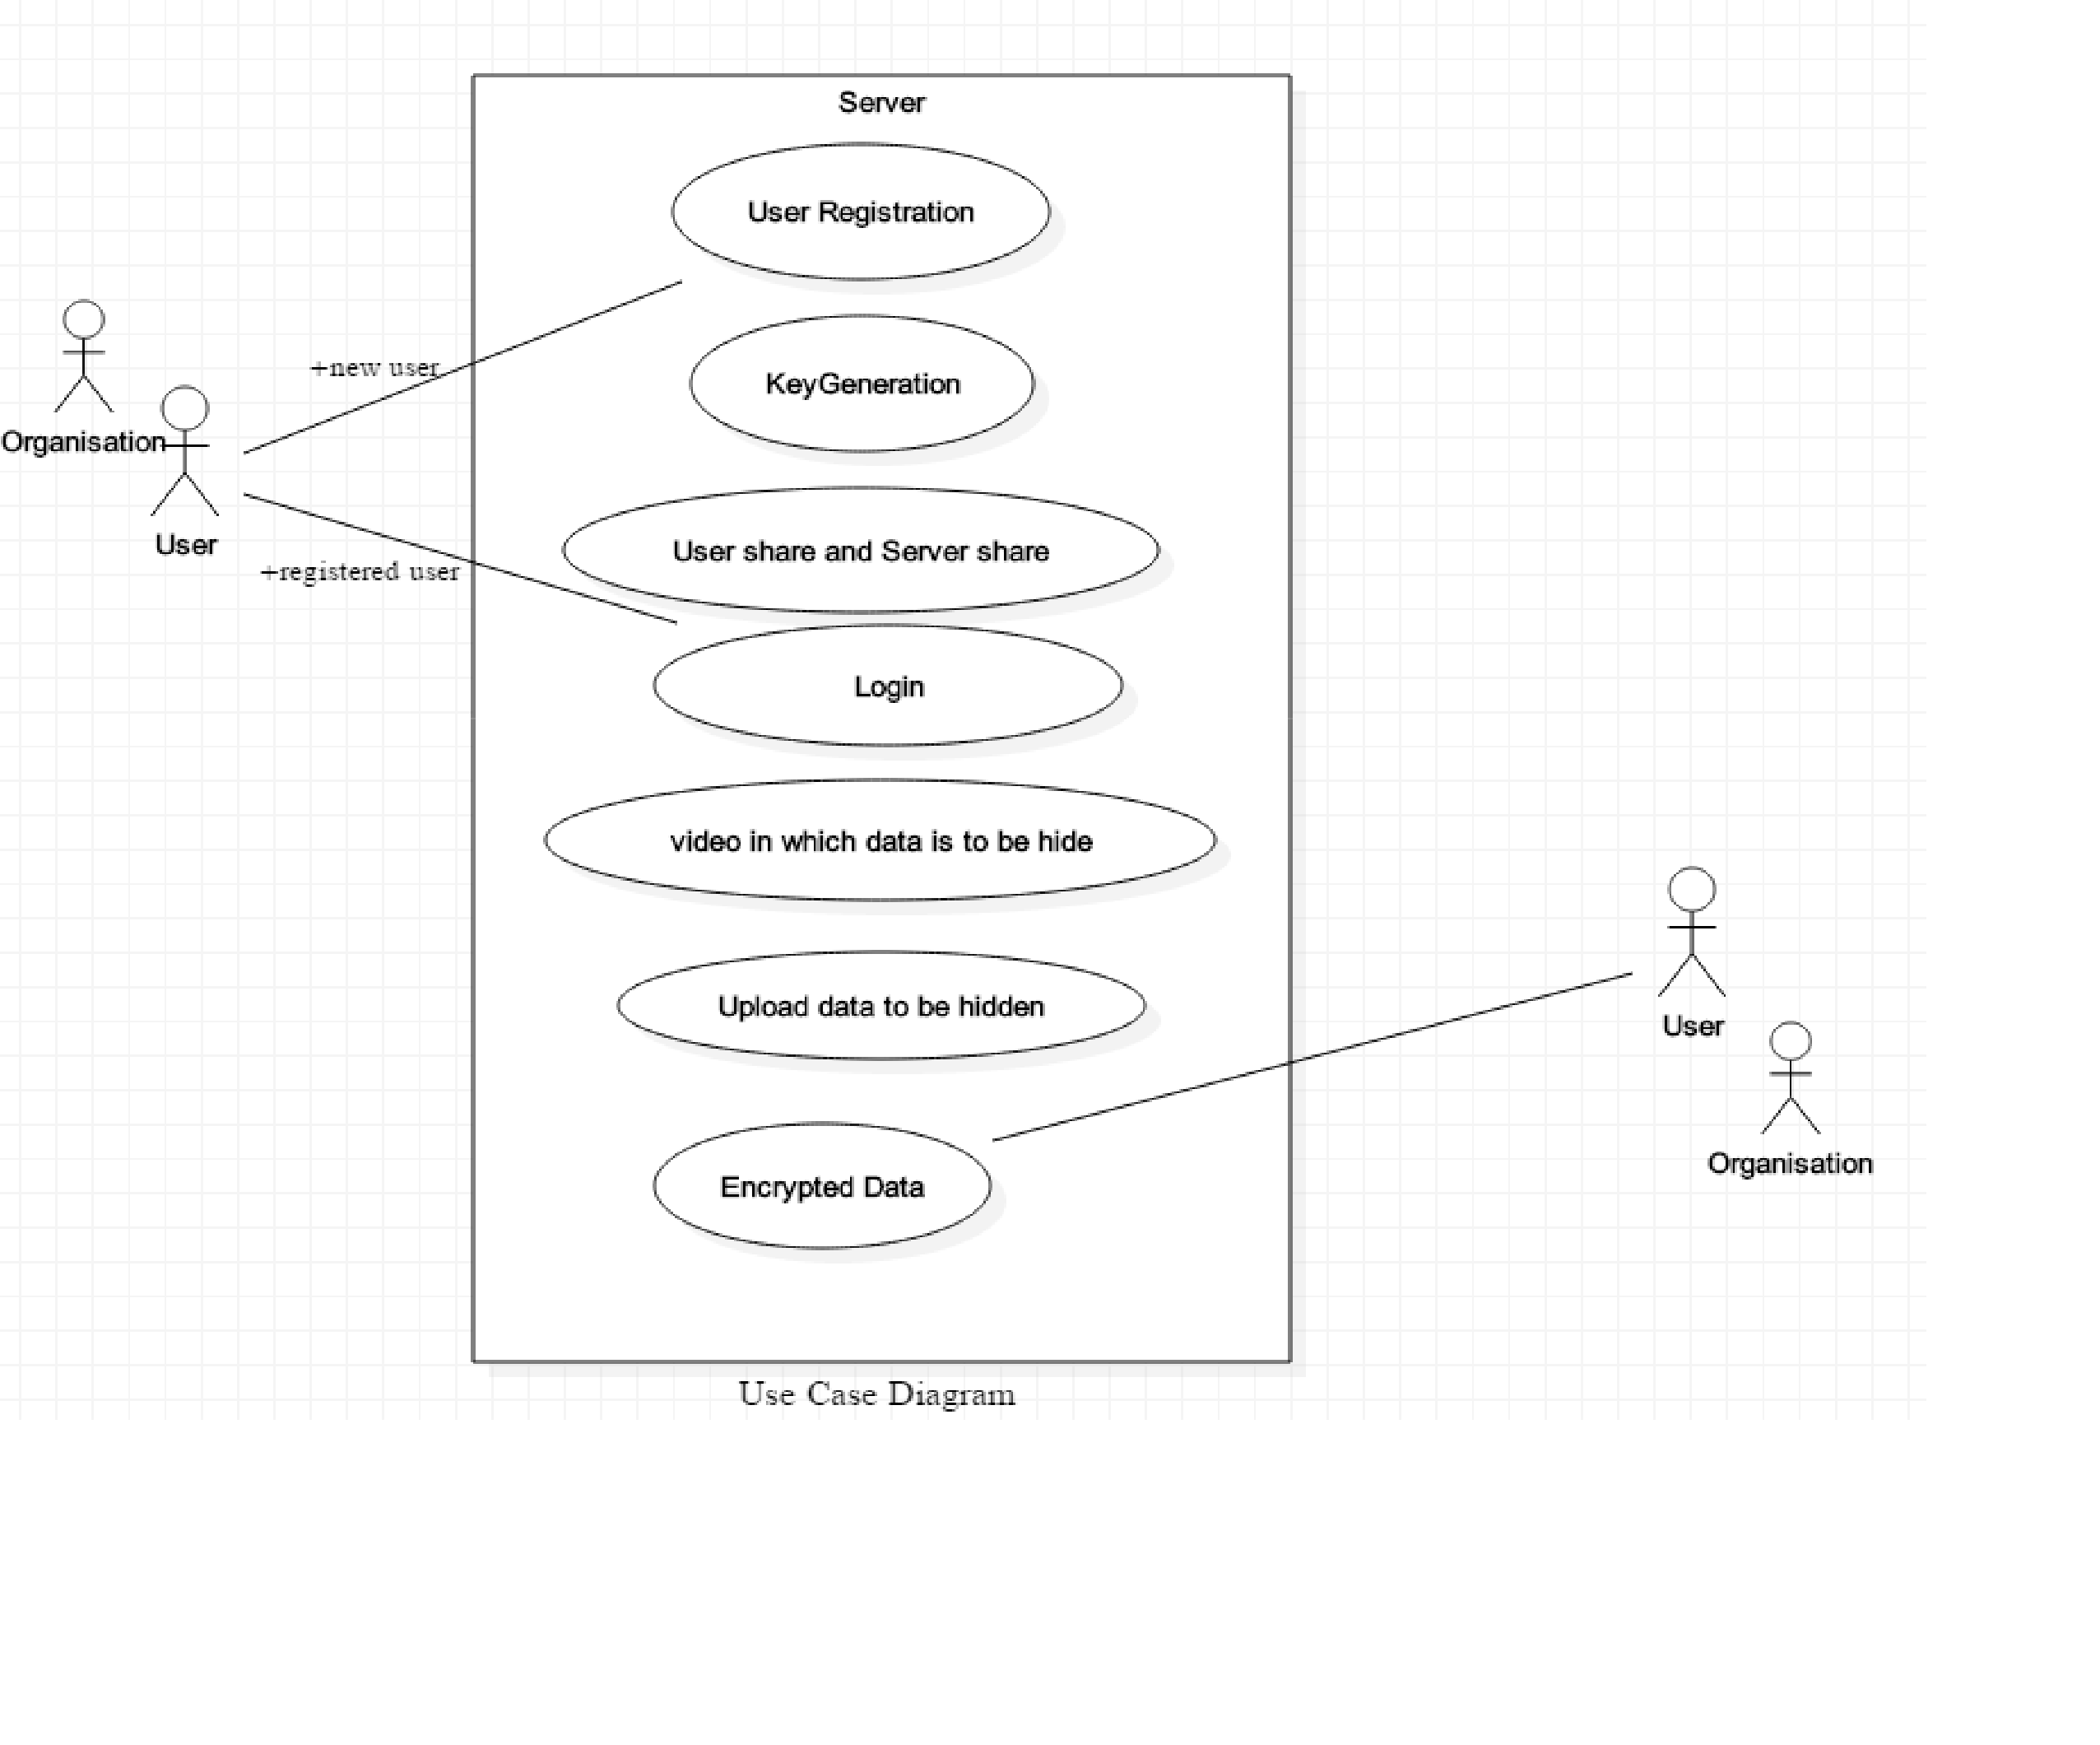
\includegraphics[scale=0.25]{usecase.png}\\
  \caption{Use Case Diagram}
  
\end{figure}
    \pagebreak
    \subsection*{DEPLOYMENT DIAGRAM}
     \begin{figure}[H]
  \centering
  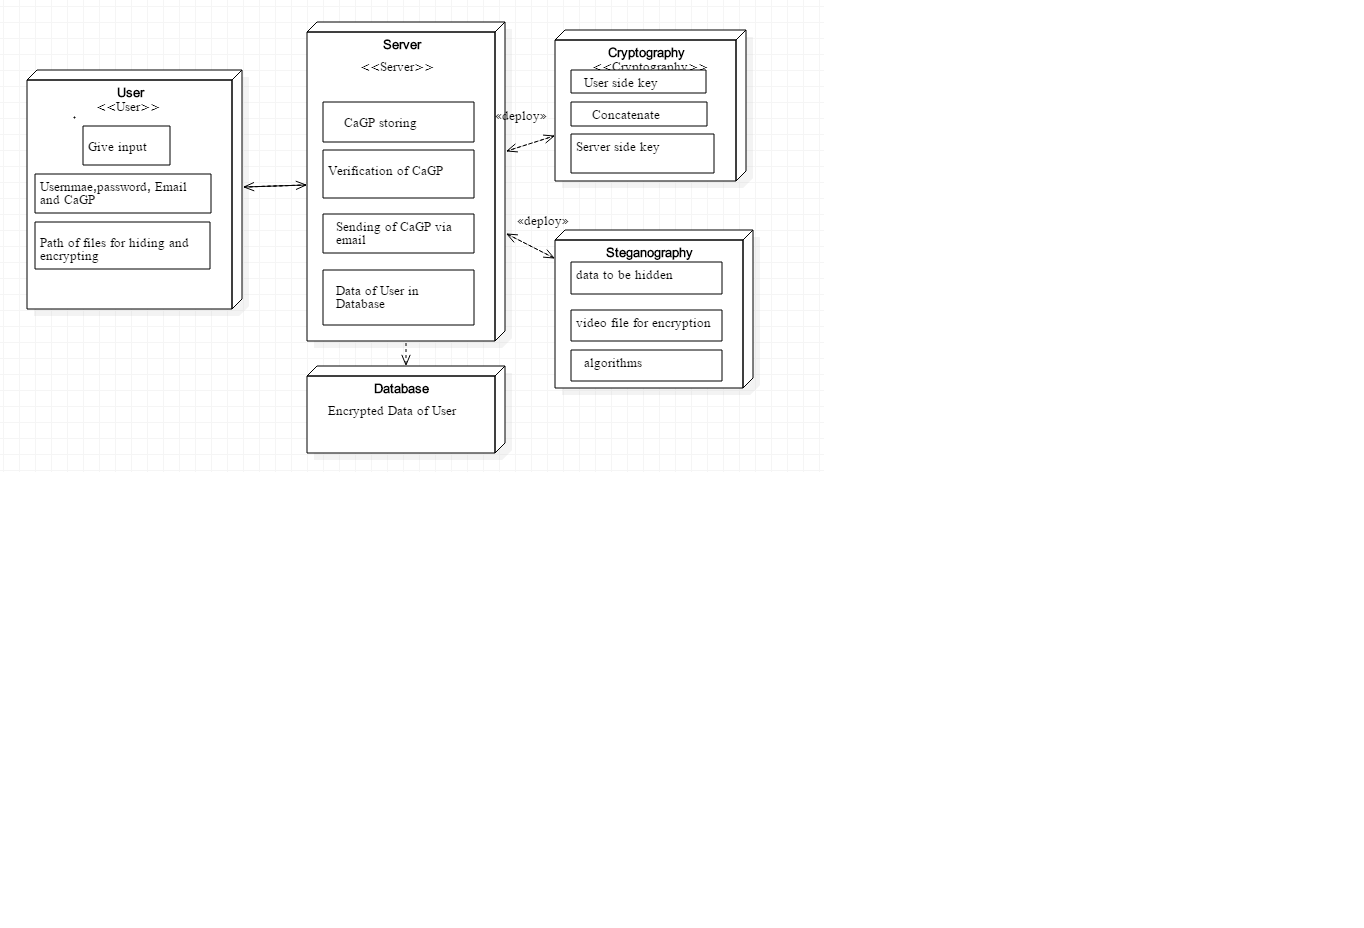
\includegraphics[scale=0.65]{deployment.png}
  \caption{Deployment Diagram}
  \end{figure}
  \pagebreak  
    \subsection*{ACTIVITY DIAGRAM}
    \begin{figure}[H]
  \centering
  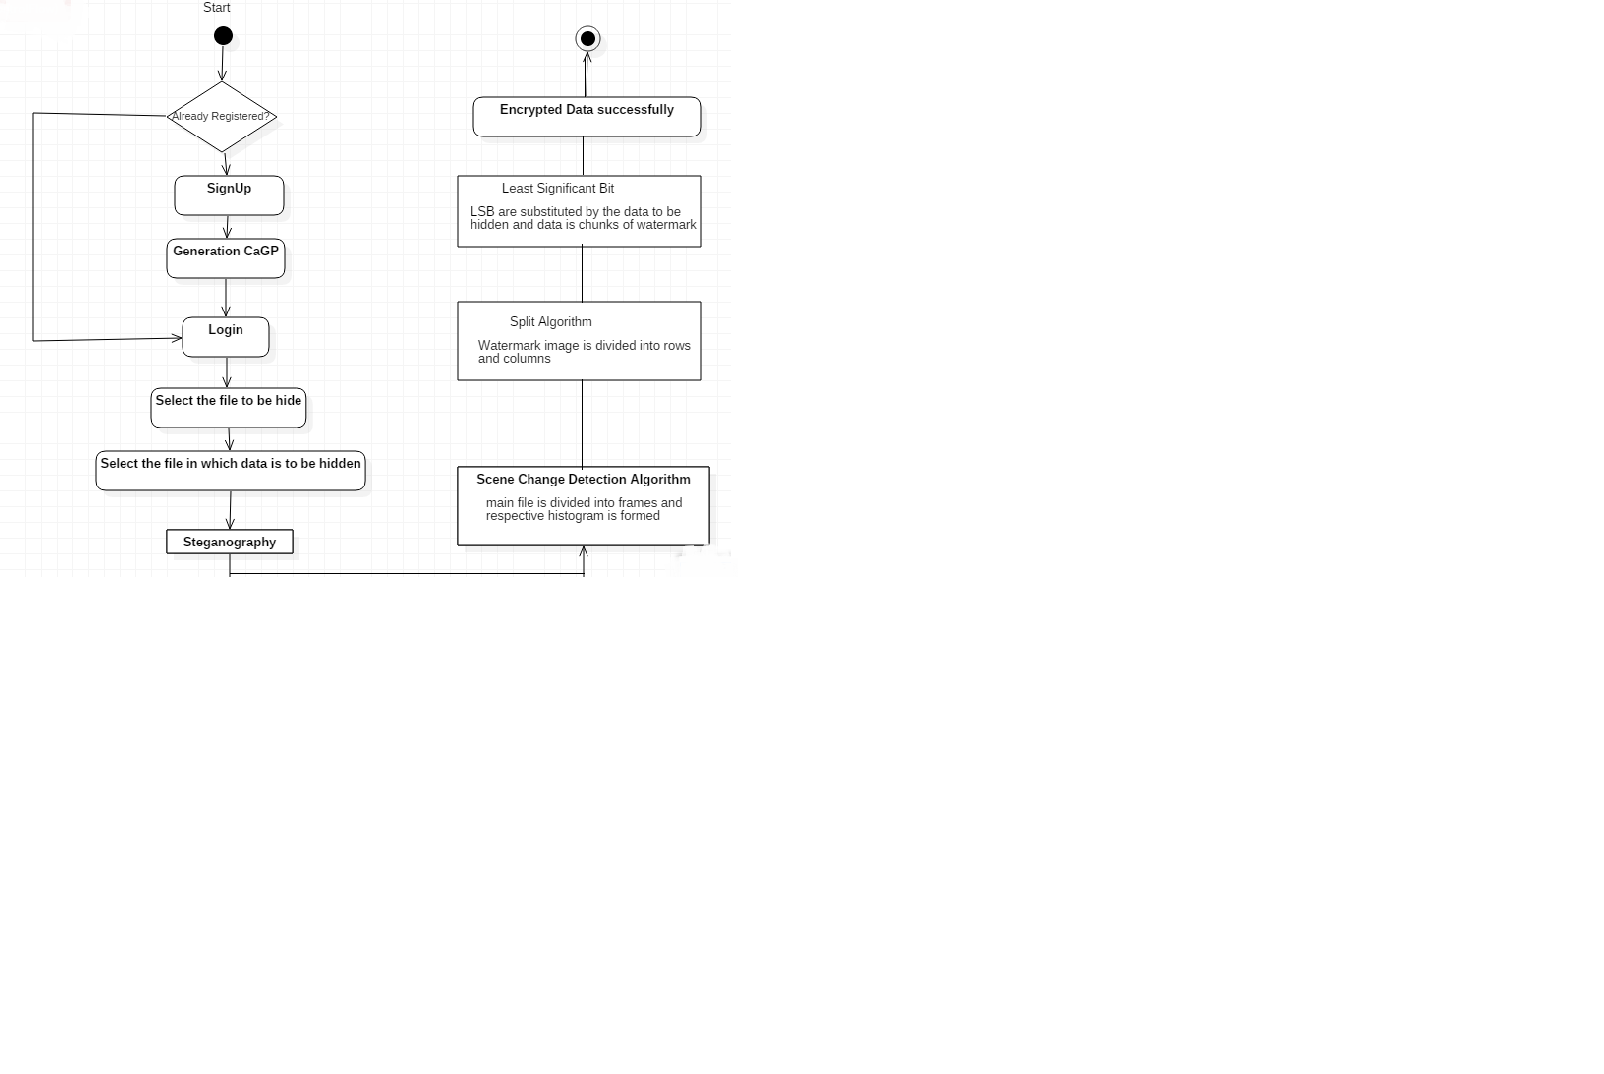
\includegraphics[scale=0.75]{activ.png}\\
  %\caption{Activity Diagram}
  
\end{figure}
    
   \pagebreak 
    \subsection*{SEQUENCE DIAGRAM}
    
    \begin{figure}[H]
  
  \centering
  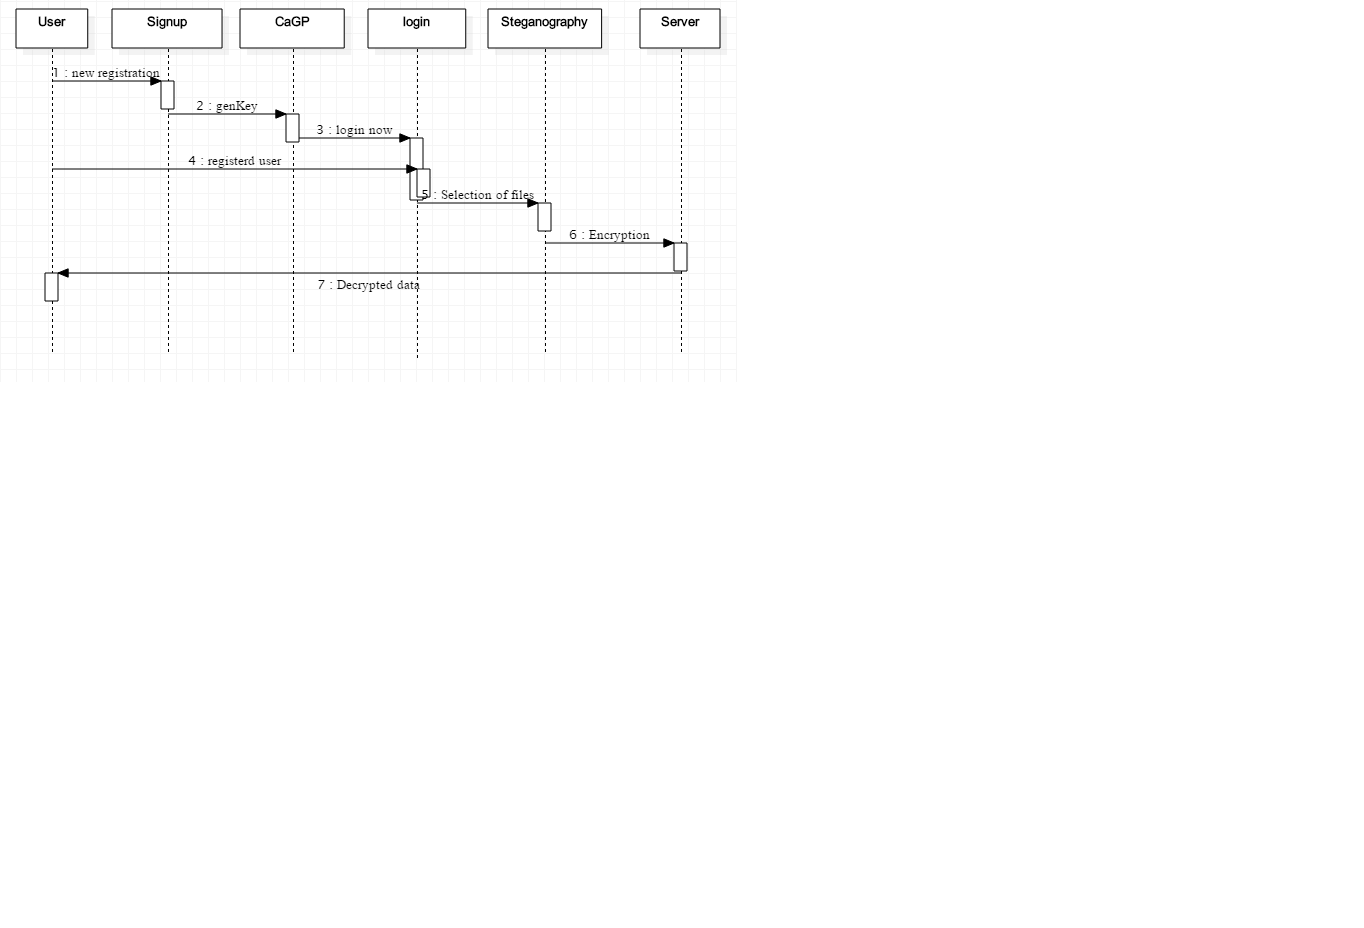
\includegraphics[scale=0.8]{sequence.png}\\
  \caption{Sequence Diagram}
  
  
\end{figure}
 \pagebreak   
    \subsection*{STATE CHART DIAGRAM}
    
    \begin{figure}[H]
  \centering
  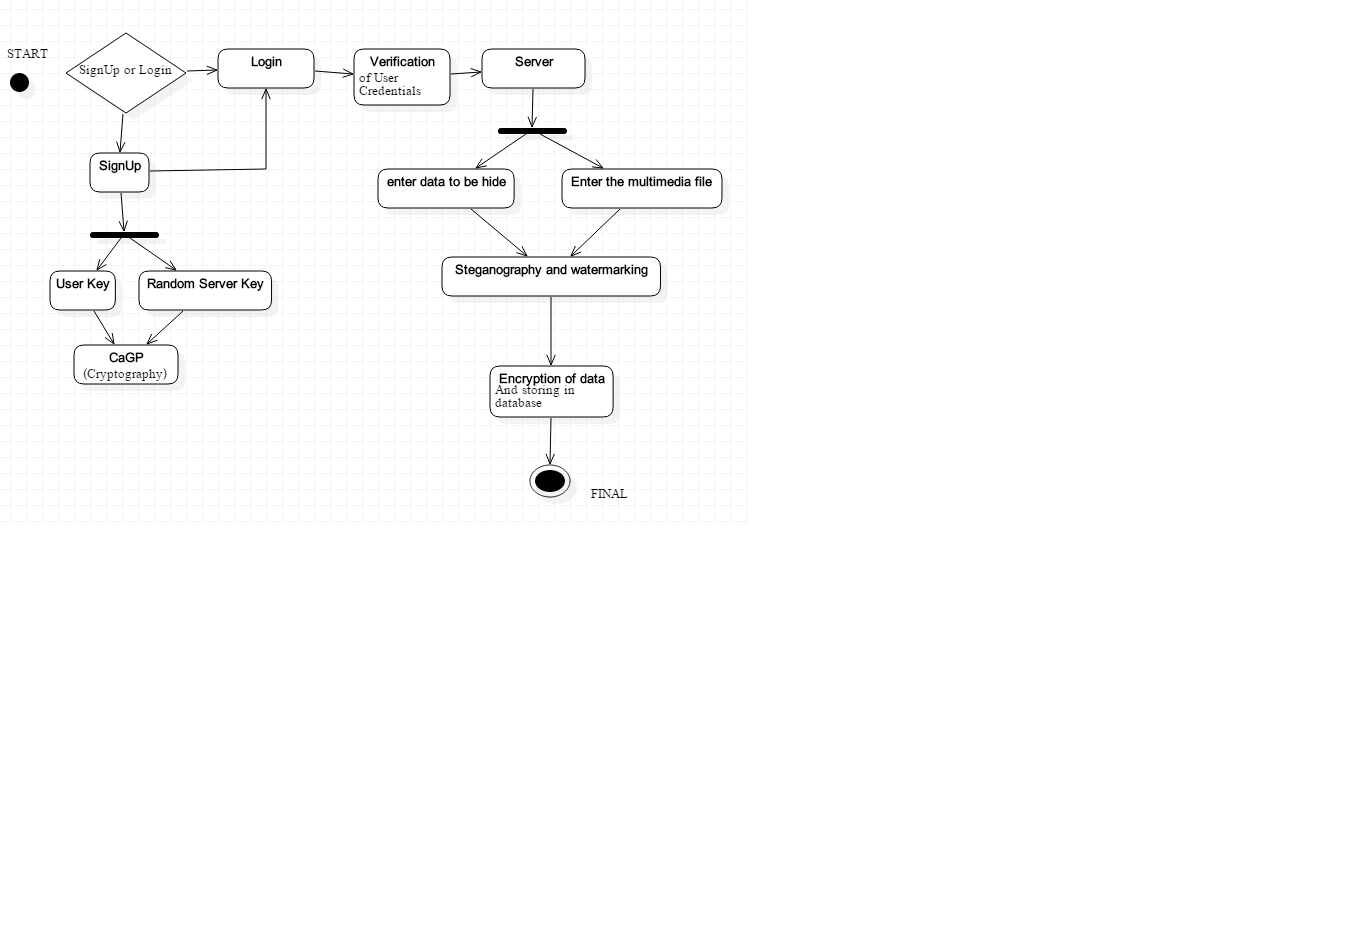
\includegraphics[scale=0.65]{State.png}\\
  \caption{State Chart Diagram}
  
\end{figure}
\pagebreak
    \subsection*{CLASS DIAGRAM}
    \begin{figure}[H]
    \centering
  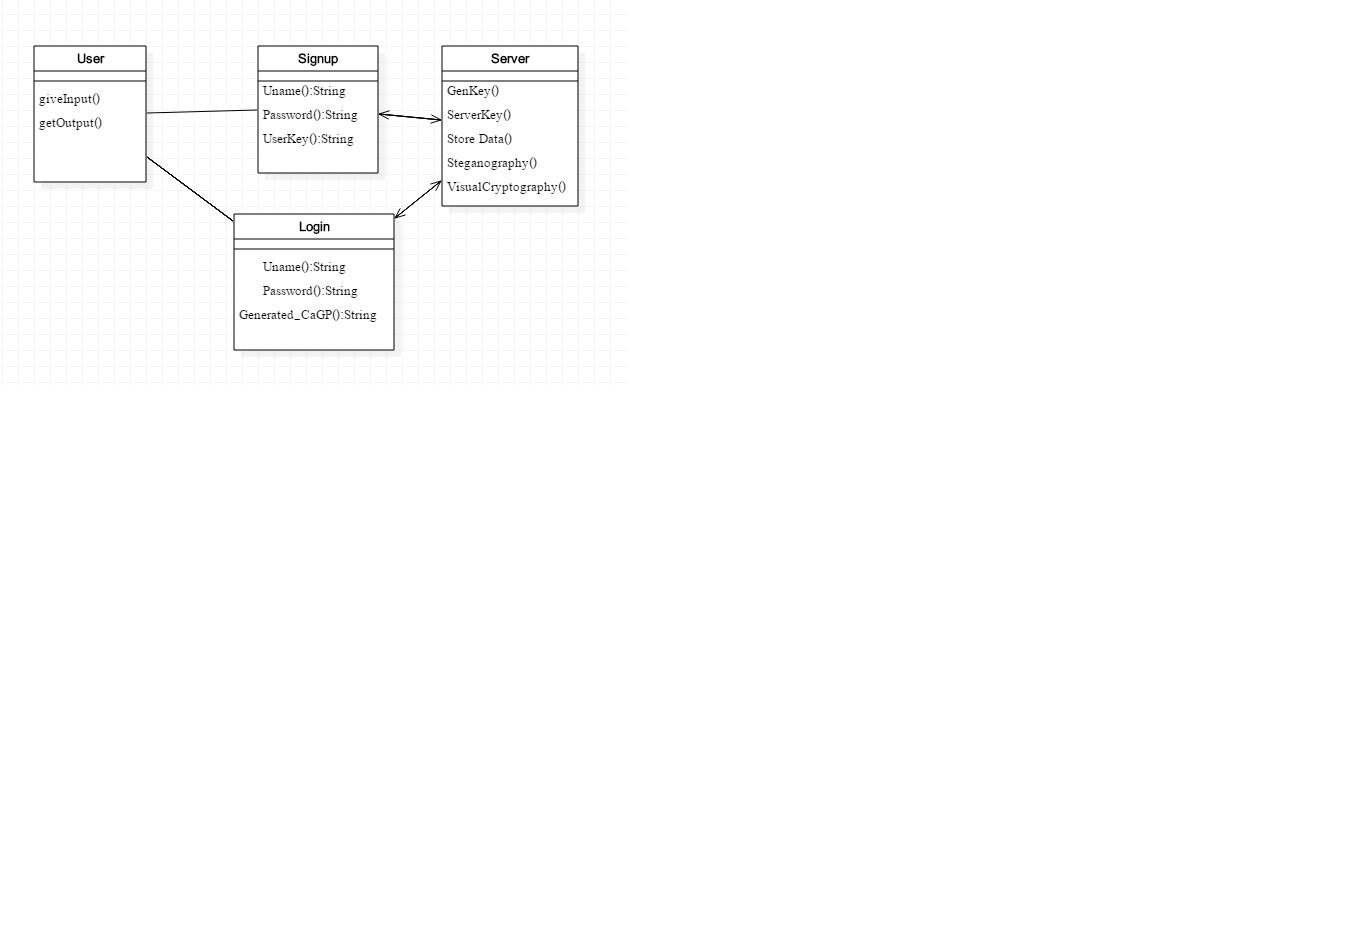
\includegraphics[scale=0.9]{Class.png}
\end{figure}


\newpage
\section*{\centering\LARGE{Lab Assignment 05}}
\subsection*{\underline{Aim}}
Testing of project problem statement using generated test data (using mathematical models, GUI, Function testing principles, if any) selection and appropriate use of testing tools, testing of UML diagram's reliability.
\noindent
\subsection*{\underline{Testing}}
\hspace{5em}Testing is a process of executing a product or application with the intention  of finding the  bugs. It can also be stated as the process of validating and verifying that a product or application meets the business and technical requirements that guided it's design and development.\\

\noindent
\begin{enumerate}
\item\textbf {Testing is about quality}
Testing is about providing a quality product to the customer.
    \begin{itemize}
    \item Quality in terms of usage.
    \item Quality in terms of look and feel.
	\item Quality in terms of data integrity.
    \item Quality in terms of security

    \end{itemize}
\item\textbf{Testing is about ideas}
Any given application can be tested in many ways. If you try out, each individual will propose a different approach and idea. We as a tester have to analyze and pick the most suitable approach.

\item\textbf{Testing is about thinking like a customer}
When we test an application, we should always think from a customer (who will use the application) point of view. Relate the flows which ideally the customer would perform on the application. Check to see if the labels/text for messages and warnings are user friendly so that the customer understands the issue if any.

\item\textbf{Testing is about coverage}
More coverage means more improved quality product. List and execute all the test combinations. Try to uncover all the odd combinations that the customer is likely to do. Prepare requirement traceability matrix. List down all the boundary conditions and negative test cases. Prioritize all the test cases.

\item\textbf{Testing is about finding defects}
Defect is described as a deviation of actual result from the requirements. This holds very true in case of testing against requirements. When checking for negative scenarios or doing ad-hoc testing we still find defects. Defects should be raised as soon as they are found and with all relevant data. People tend to miss out raising defects assuming that they are minor or just UI. Every valid defect which gets fixed adds to the quality of the product.

\item\textbf{Testing is about simplicity}
There is no point in building an application which is of high complexity and of no use. Rather we should suggest for simple design which even a lay man can use. Suggest for enhancements in the system. Users will always prefer using a system which is less complex and easy to use and understandable.

\item\textbf{Testing is about collaboration}
Testing is an activity which cannot be performed all alone.It always has to be in collaboration with the other teams like requirement, design, development, process etc.

\item\textbf{Testing is about documentation}
Documentation plays a major role in testing phase. Document the test scenarios, test cases. Prepare traceability matrix. Prepare checklist of test activities done. Prepare checklist of UI testing done. Capture all the screenshots/evidences. These documents will be very useful in future for reference in case someone has to do a round of testing again. Document all the defects in any means Microsoft Excel or defect management tool. Document the test data, environment details etc. as well.

\textbf{Testing is about time management }

Defect found later in test cycle impacts the cost and time. If we can uncover more critical defects initially in the test cycle, the more time we get to test it better. Testers always have a challenge in time management. We have to prepare the test data upfront, recreate the test data in case of failures. Track defects, test case status, check for regressions all in parallel. This makes time management really a challenge for us.


\end{enumerate}

\subsection*{\underline{Testing types}}
It describes which testing types we might follow in our testing life cycle. Here we are using:
\begin{itemize}
\item \textbf{Black Box Testing}\\
Internal system design is not considered in this type of testing. Tests are based on requirements and functionality.\\
 In our project black box testing can be used for testing:


\begin{itemize}
\item Incorrect or missing function
\item	Interface errors
\item	Errors in data structure or external job access
\item	Performance errors
\item	Initialization and termination errors.
 
\end{itemize}

In the proposed application with the help of this technique, we do not use the code to determine a test suite; rather, knowing the problem that we are trying to solve, we come up with four types of test data: 
\begin{enumerate}
\item	Easy-to-compute data,
\item	Typical data,
\item	Boundary / extreme data,
\item	Bogus data.

\end{enumerate}
But in our application we does not provide any external data, the role of user is only to give number of nodes for formation of clusters and for the formation of sink node.


\item \textbf{White Box Testing}\\
This testing is based on knowledge of the internal logic of an application’s code. Also known as Glass box Testing. Internal software and code working should be known for this type of testing. Tests are based on coverage of code statements, branches, paths, conditions.\\

In our project white box testing will be used in the implementation stage to check the android application coding and to check whether the app is connected with the database efficiently so that there is no wrong data updated in the database which the society member won’t agree with. The images should be updated automatically so that next time there is no error in validating the visitor. All this implementation should be checked in the code.




\item \textbf{Unit Testing}\\
Testing of individual software components or modules. Typically done by the programmer and not by testers, as it requires detailed knowledge of the internal program design and code. may require developing test driver modules or test harnesses.\\
In our project there are 4 modules. They are. These modules should be tested individually and the defects must be resolved before starting integration testing of these modules.


\item \textbf{System Testing}\\
Entire system is tested as per the requirements. Black-box type testing that is based on overall requirements specifications, covers all combined parts of a system.\\
   In the entire society management system as a whole, the end user requirements will be:
\begin{enumerate}
\item Maintainance of all records online.
\item Updating and choosing their activities such as casting a vote, Advertising their flat for sale, Money transaction from their accounts etc.
\item Appropriate display of vacant slots and parking of the vehicle in that slot.
\item Face detection of the visitor along with details to be stored in database and displayed on the application.
\end{enumerate}




\item \textbf{Integration Testing}\\
Testing of integrated modules to verify combined functionality after integration. Modules are typically code modules, individual applications, client and server applications on a network, etc. This type of testing is especially relevant to client/server and distributed systems. In Integration testing      will be combined and again tested and if any error in the applications on the network will be resolved.
\item \textbf{Functional Testing}
This type of testing ignores the internal parts and focus on the output is as per requirement or not. Black-box type testing geared to functional requirements of an application. The final output of our project is the proper parking of vehicles and face detection and comparison with existing images in the database.
\item \textbf{GUI Testing}

\end{itemize}

\begin{table}[ht]

\begin{tabular}{ |M{4cm}|p{5cm}|M{2.5cm}|M{3.2cm}|  }
 \hline
 \textbf{USE CASE} & \textbf{FUNCTION BEING TESTED} & \textbf{INPUT} & \textbf{EXPECTED OUTPUT}\\
 \hline
 
Data Collection & Is data collected properly? & Web data & Stored records in DB\\

\hline
 Data Classification & Is data classified into  classes as per attributes? & Data in DB & Classes of attributes\\
 
 \hline
 Pattern identification & Is unique patterns generated? & Classes from classifier & Patterns as rules.\\
 
 \hline
 Prediction & Is regions having a common pattern? & Rules from apriori & Expected output\\
  
  \hline
  
 
 \end{tabular}
 \begin{center}
 \caption{Test Cases}
 \end{center}
 \end{table}